%!TEX root = ../thesis.tex
%*******************************************************************************
%****************************** Third Chapter **********************************
%*******************************************************************************
%Here you make the strongest statement concerning observations. Highlight the information you want readers to remember. Explain how the results correlate with the problems you have indicated in the introduction. Describe all new things that are significant in finding a solution.

%The recommendations part is for giving advice and indicating other actions that will help to solve particular problems. Sound your own opinion about the direction of future research. Most of the time you have to write it. Just like a research proposal.

%Acknowledgments part is a paragraph where you mention everyone who helped you with composition. Place all cited and used information resources into one list or form an annotated bibliography if needed.
\chapter{Methodology}

% **************************** Define Graphics Path **************************
%\ifpdf
%    \graphicspath{{Chapter3/Figs/Raster/}{Chapter3/Figs/PDF/}{Chapter3/Figs/}}
%\else
%    \graphicspath{{Chapter3/Figs/Vector/}{Chapter3/Figs/}}
%\fi
In this section, we will introduce the proposed edge-to-cloud sysem for surveillance video analytics applications in details. And then, the our approach for moving objects detection in compressed-video domain is presented. In addtion, we will introduce the performance evaluated model for video analytics platform used in this study. 

\section{The edge-to-clound architecture for Surveillance Applications}
\begin{figure*}
\centering
 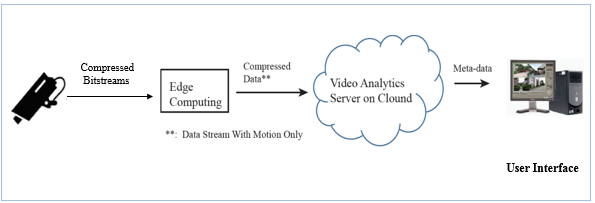
\includegraphics[width=1.0\linewidth]{Figures/arch.png}
 \caption{ Our proposed system.}
 \label{fig:arch}
\end{figure*}
There is a trend to offload computation from the cloud to the edge where the data is generated. To minimize bandwidth consumption, and improving energy efficiency, edge computing has been used. “Edge computing performs data processing at the edge of the network, close to the data source. For network cameras, a camera source node can forward its video task to nearby edge nodes via local wireless/wire-link networks”. The camera captures the video sequences and divides each of them into multiple video trunks, compresses them and stream to edge nodes. Next, edge nodes implement video processing functions on the received video trunks and upload the results to a cloud server for further video analysis (such as object/event detection). In this study, as shown in Figure \ref{fig:arch}, we consider an edge computing network, which comprises three primary components, namely, camera source node, edge node, and cloud server.
\begin{itemize}
\item “Camera source node where the camera node periodically generates video tasks: compresses video chunks at certain compression ratios, and then allocate compressed video chunks among all edge nodes according to specific scheduling policies”.
\item “Edge node where the edge helps preprocess video chunks: moreover, edge nodes can cooperative groups based on specific group formation policy”.
\item “Cloud Server: cloud server collects the preprocessing results from edge nodes: video analytics server has enough computational abilities, and performs additional video analysis”.
\end{itemize}
 “During a sparse edge node deployment, an edge node  connect to one camera  at a certain location; however, in a dense deployment, an edge node may have multiple connection with multiple cameras. In this study, we focus on reducing processing load on cloud server by minimizing the video chunks that are forwarded from camera sources. Therefore, an edge device runs preprocessing tasks to filter uninteresting video chunks. The \textbf{term uninteresting video chunks} is defined via scenario specification: In this study, it is static scenes without any objects and gradual changes” (Nguyen Van Dien and Jaehyuk Choi, 2020, p.8).

\section{The Proposed Method of Moving Object Detection in Compressed Domain}
\begin{figure*}
\centering
 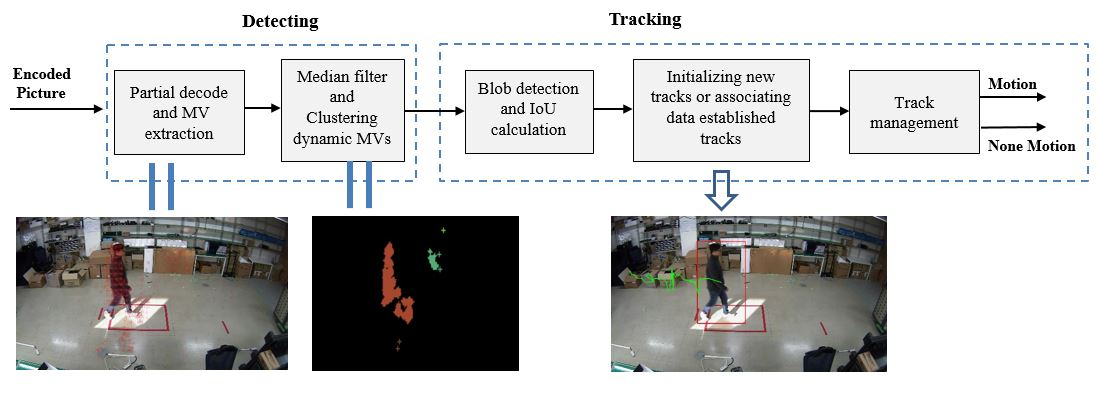
\includegraphics[width=1.0\linewidth]{Figures/arch.jpg}
 \caption{The proposed method for moving object detection in compressed video domain.}
 \label{fig:proposedMethod}
\end{figure*}
\begin{figure*}
\centering
\subfloat[]
{
    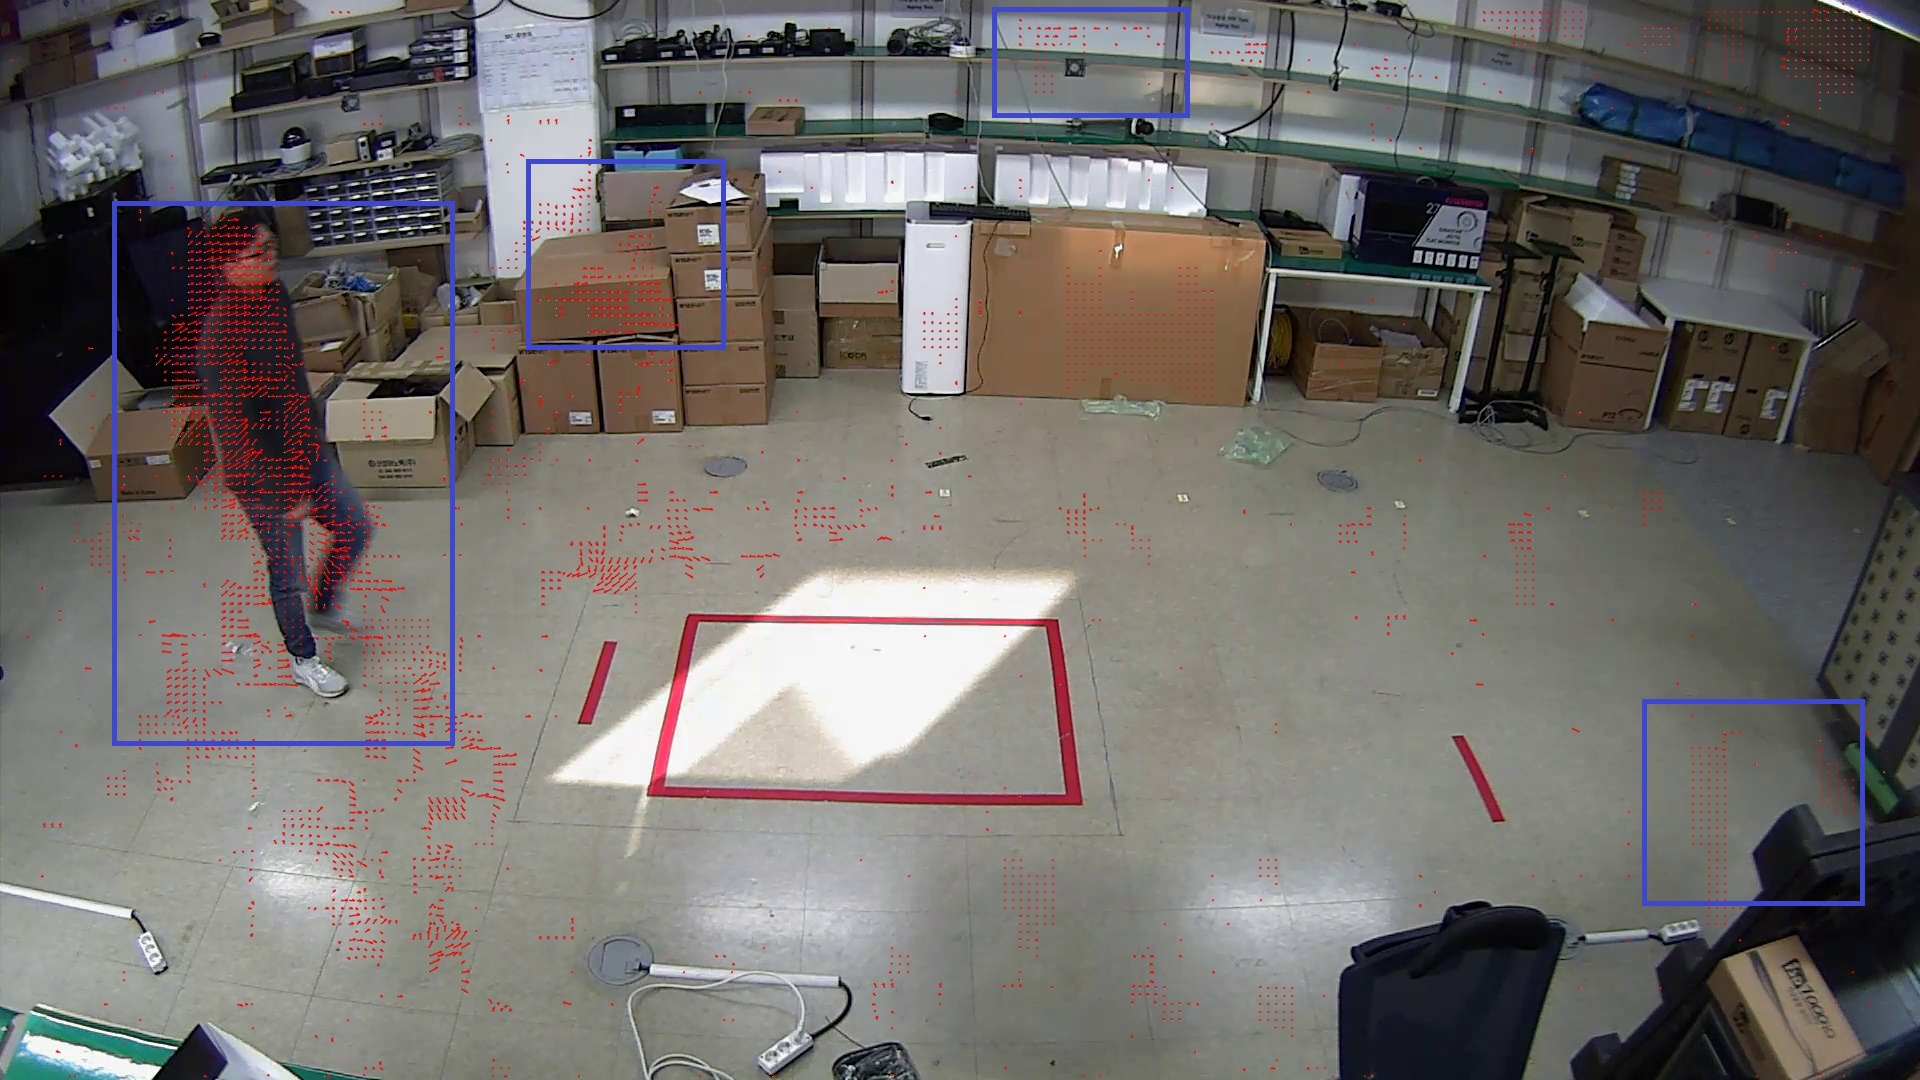
\includegraphics[width=0.3\linewidth]{Figures/1340.jpg}
}
\subfloat[]
{
    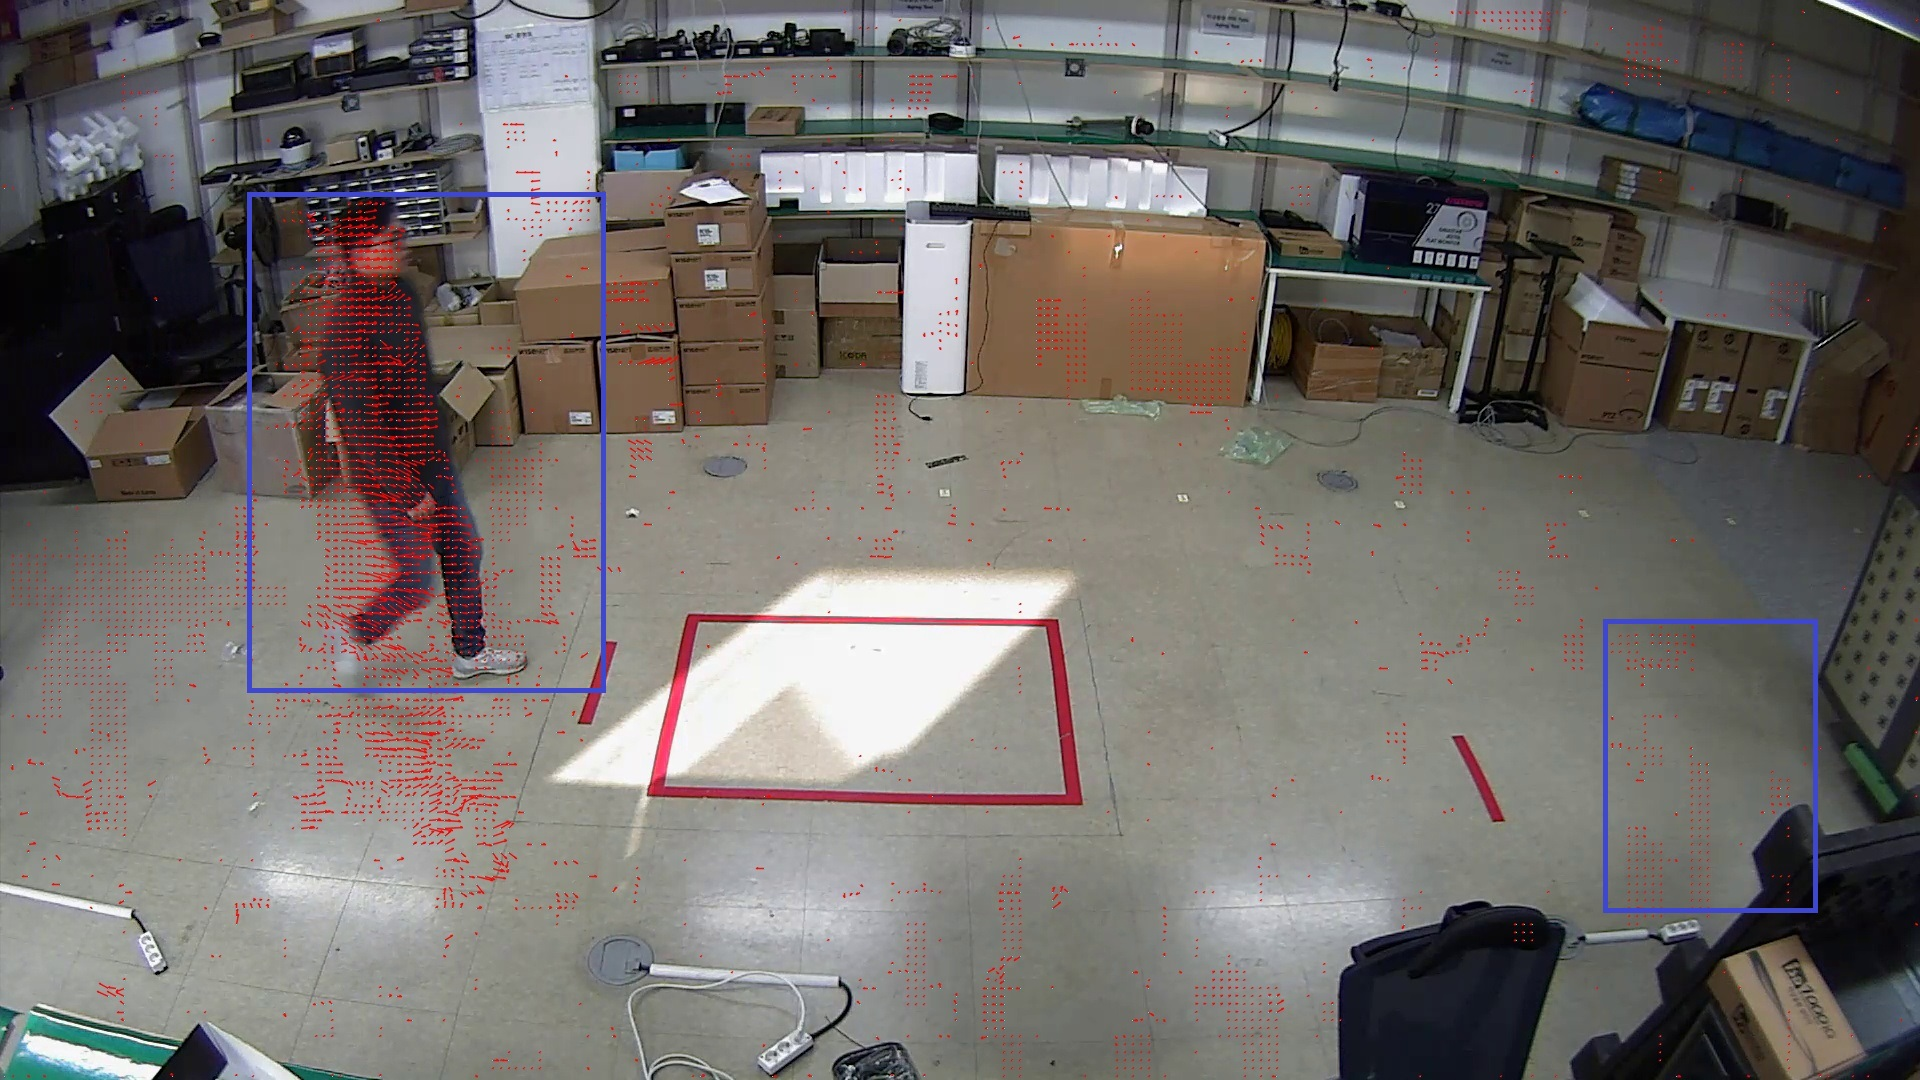
\includegraphics[width=0.3\linewidth]{Figures/1350.jpg}
}
\subfloat[]
{
    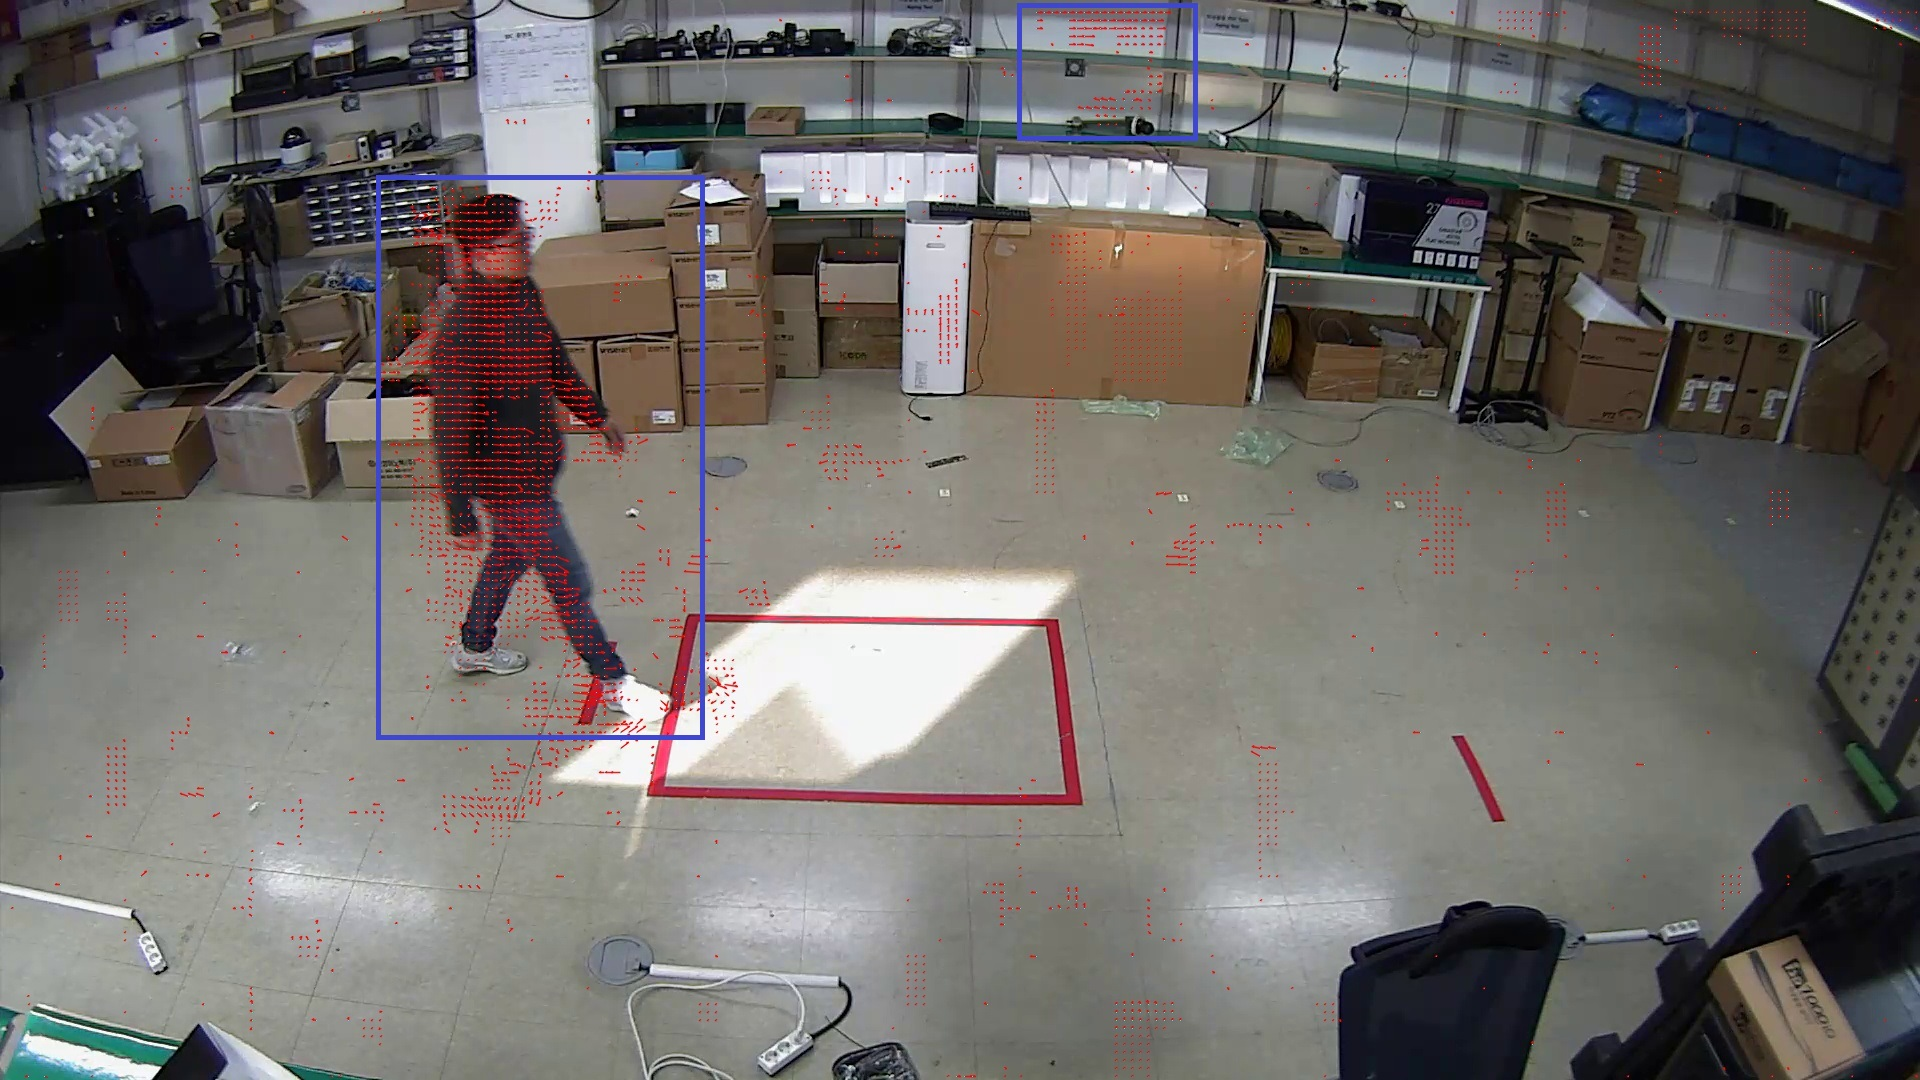
\includegraphics[width=0.3\linewidth]{Figures/1360.jpg}
}\\
\subfloat[]
{
    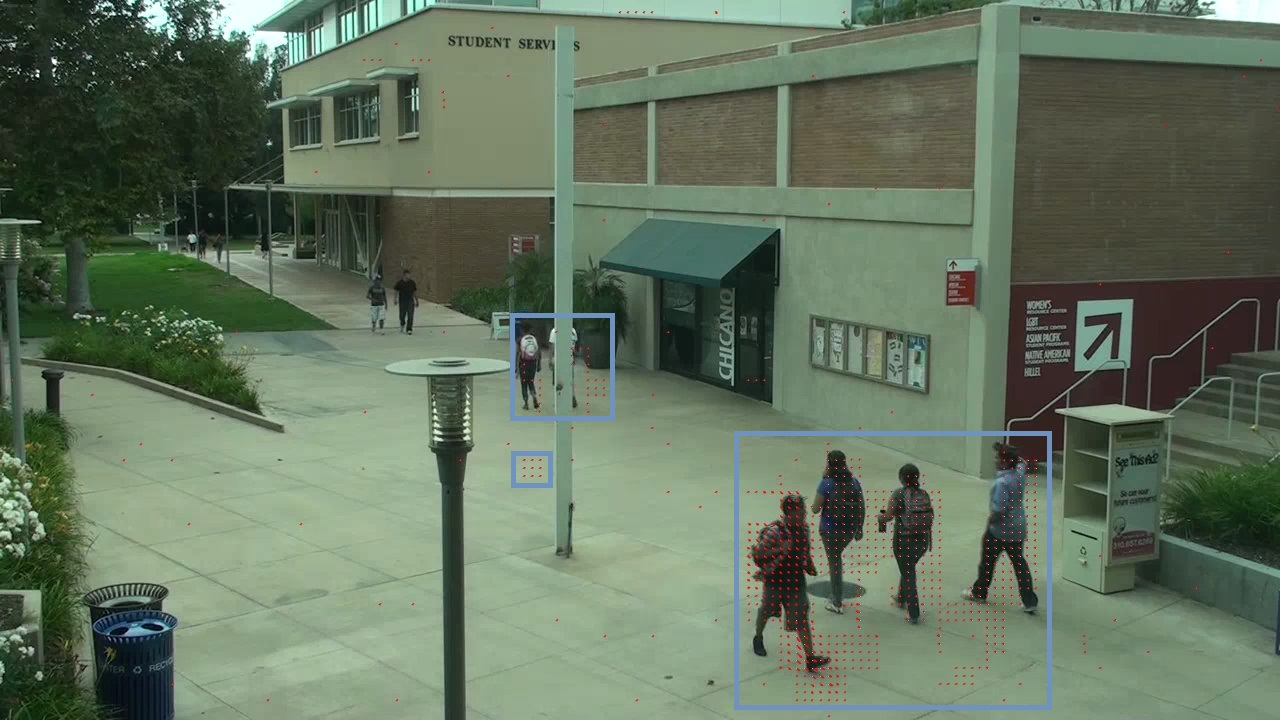
\includegraphics[width=0.3\linewidth]{Figures/3.jpg}
}
\subfloat[]
{
    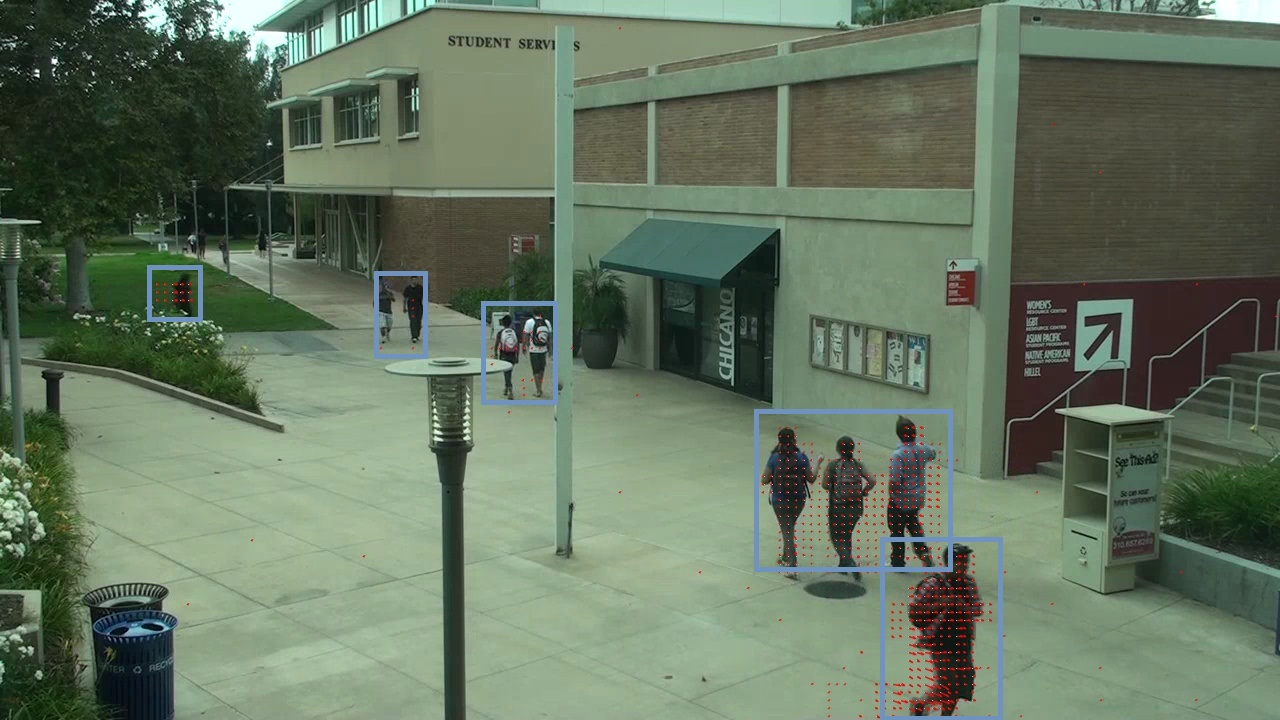
\includegraphics[width=0.3\linewidth]{Figures/35.jpg}
}
\subfloat[]
{
    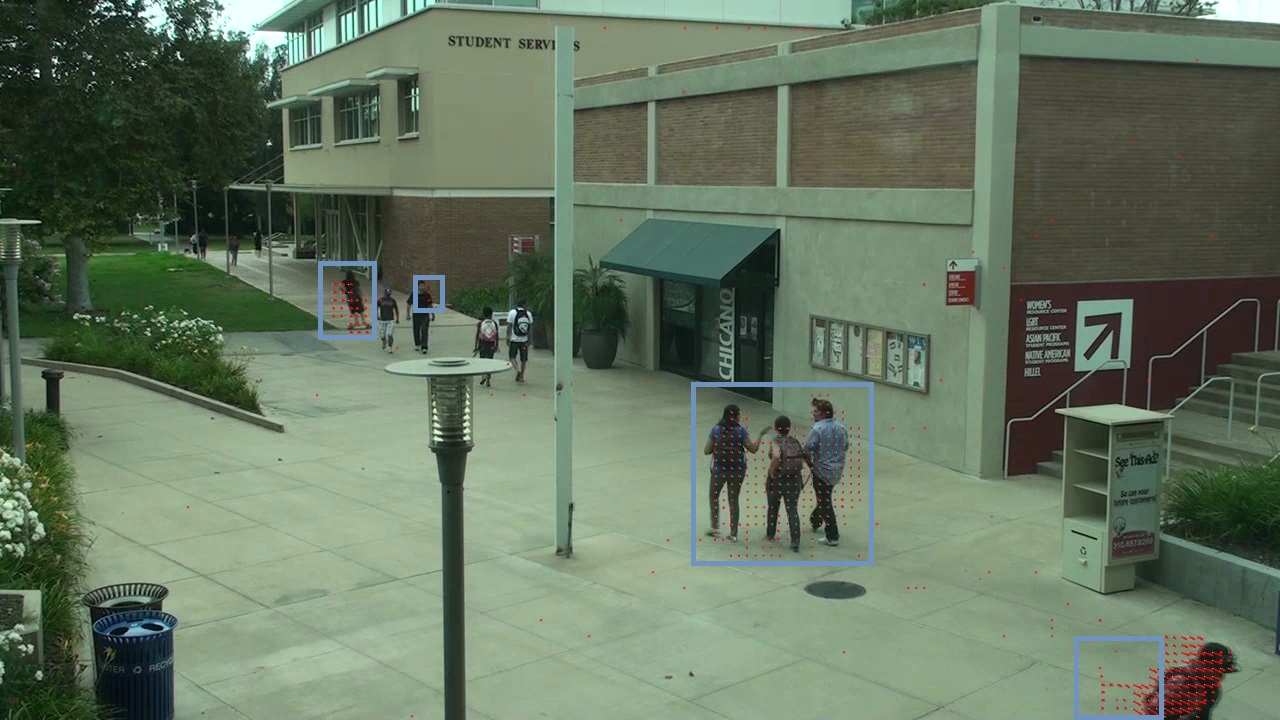
\includegraphics[width=0.3\linewidth]{Figures/70.jpg}
}
\caption{The video coding MV extraction from consecutive frames with two different test sequences.}
\label{fig:mvextract}
\end{figure*}
MV represents the changes between video frames may caused by:
\begin{itemize}
\item Object motion (car, human activity)
\item Camera motion (panning, tilt, zoom, rotation).
\item Lighting condition changes
\end{itemize}
The MV group generated by lighting change, normally randomly occur without following any certain flows and have various sizes. The MV group generated by human motion (walking, running),  move in certain direction and It’s size is similar with object size in video frame. This observation is good factor to classify MVs into real-motion and noise motion group. “The aim of this method is to analyze only MVs at the edge device, recognize the real moving objects, and exclude the noised motions that are generated by environmental factors such as illumination changes and background movement, in the current video scene. For this purpose, we propose a method that has a workflow shown in Figure \ref{fig:proposedMethod} to analyze the video coding MVs. In order to obtain MVs from compressed bitstream, the input video stream is partially decoded and the collected MVs consist of both real object MVs and noise MVs. The example of extracted MVs are represented in Figure \ref{fig:mvextract} in consecutive frames of two different video test sequences. To analyze these MVs, the following functionalities are involved” (Nguyen Van Dien and Jaehyuk Choi, 2020, p.8).
\subsection{Motion Vector Median Filter and The Moving Object Detection}
\label{sub:filter}
\begin{figure*}
\centering
\subfloat[]
{
    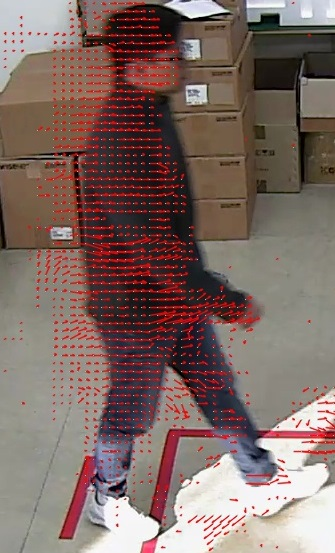
\includegraphics[scale=0.325]{Figures/1327_mv.jpg}
}
\subfloat[]
{
    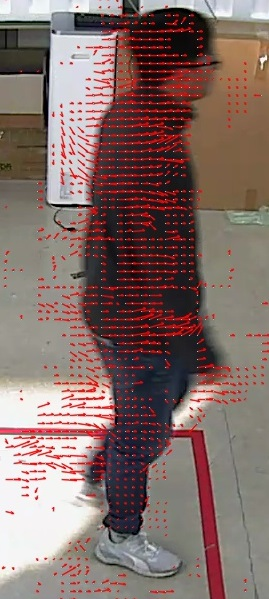
\includegraphics[scale=0.3]{Figures/1350_mv.jpg}
}
\subfloat[]
{
    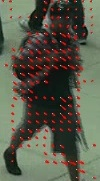
\includegraphics[scale=1.0]{Figures/30_mv.jpg}
}
\subfloat[]
{
    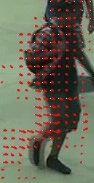
\includegraphics[scale=1.0]{Figures/10_mv.jpg}
}
\caption{Motion vector of a moving object in different video test sequences: (a, b) our record video, (c, d) Test video in VIRAT}
\label{fig:mvobject}
\end{figure*}
The compressed-domain MVs may not present the actual of true motion due to the properties of motion estimation as shown in Figure \ref{fig:mvanalysis}(a,e). Therefore, it is desirable to remove motion vectors that can be categorised as false case for moving objects detection. We found that “MVs  whose magnitudes are very low, compared to the other MVs related to the real moving object, has to be replaced with the median value of neighbouring MVs. Therefore, the application of vector median filter aims to eliminate isolated vector noises and smoothen the difference of MV between adjacent blocks”(Nguyen Van Dien and Jaehyuk Choi, 2020, p.9). \\ Because H.264/AVC allows for variable-sized block partitioning, we construct a uniformly sample MV field by mapping all MVs to 4x4 blocks. “Theoretically, the motion vector average (the normalized vector) among all elements $N_{mv}$ in NxN (N=4 is chosen in this study) window function is calculated by Equation \ref{eqn:1}: 
\begin{equation}
\label{eqn:1}
N_{mv}= \frac{\sum_{i=1, j=1}^{N*N}MV_{ij}}{N*N}
\end{equation}          
Where: $MV_{ij}$ is the MV elements in the N×N window. Finally, the smoothened motion filter is presented, which is experimentally determined as shown in Figure \ref{fig:mvanalysis}(b,f) using the input MV, including isolated motion vectors noise, are smoothened in the areas that mostly correspond to the object boundaries. In order to detect the moving objects, a cluster detector is involved to define the number of moving objects and their positions in the image. Then, a density-based cluster technique is used to completely segment the moving objects. The first step, MV whose magnitudes can be used to easily extract moving objects from the background. However, it is difficult to directly and completely segment moving objects because not all MVs on the objects have the same motion state. While every part of a rigid body maintains nearly the same motion state, different parts of a non-rigid body can move in various ways”(Nguyen Van Dien and Jaehyuk Choi, 2020, p.8) (see Figure \ref{fig:mvobject}). “In order to cluster detected MVs into dynamic clusters, a range search algorithm based on the euclidean distance of the MV point is used, under the presumption that dense points represents the same object. It requires a parameter $\varepsilon$ where $\varepsilon$ is the spatial distance threshold between density reachable MV. The goal is to partition \textit{n} MV points $\chi \subset \mathbb{R}^{d}$ into \textit{k} clusters using k-means filter. Each of the \textit{n} data points will be assigned to a cluster with the nearest mean. The mean of each cluster is called its \textit{center}. For the k-means problem, we wish to choose \textit{k} centers $\mathbb{C}$ so as to minimize the potential Equation \ref{eqn:cluster}: \\
\begin{equation}
\label{eqn:cluster}
\phi = \sum_{x \in \chi}^{}\underset{c \in \mathbb{C}}{min}\left \| x - c \right \|^{2}
\end{equation} 
From these centers, we can define a clustering by grouping data points according to which center each point is assigned to. With MV points, following steps are performed frame by frame:
\begin{itemize}
\item For each $p_{i} \in \chi$, find all the neighboring points within spatial distance $\varepsilon$.
\item Cluster all the MV points that are density reachable or density connecting \cite{ester1996density} and label them.
\item Terminate the process after all the MV points are checked. The output is a set of clusters of dynamic points.
\end{itemize}
The distance threshold $\varepsilon$ decides the range of density reachability \cite{ester1996density}”(Nguyen Van Dien and Jaehyuk Choi, 2020, p.10).
\begin{figure*}
\centering
\subfloat[]
{
    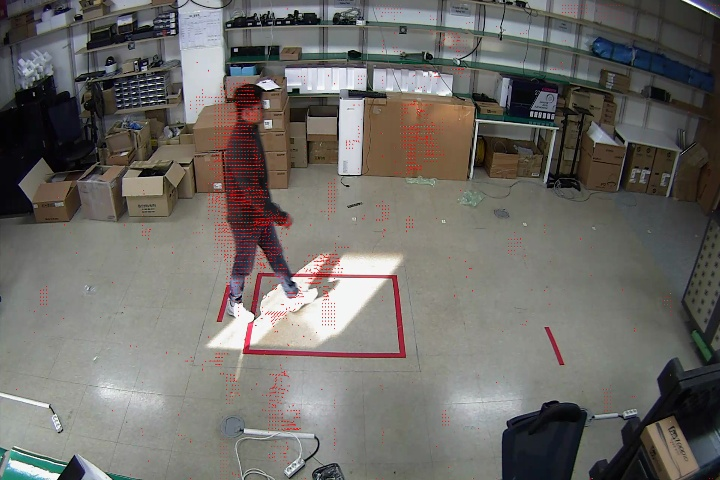
\includegraphics[width=0.25\linewidth]{Figures/1328_mv.jpg}
}
\subfloat[]
{
    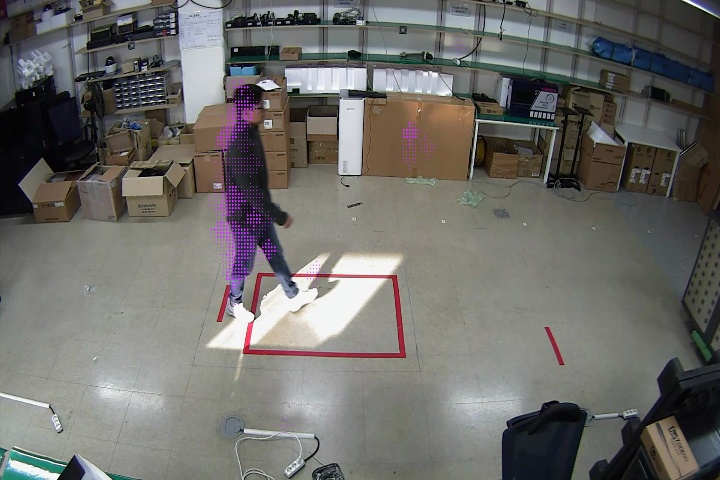
\includegraphics[width=0.25\linewidth]{Figures/1328_occ.jpg}
}
\subfloat[]
{
    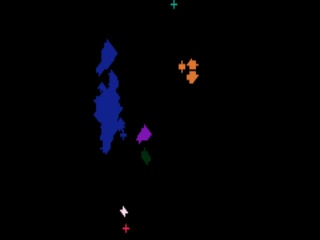
\includegraphics[scale=0.3]{Figures/1328_res.jpg}
}
\subfloat[]
{
    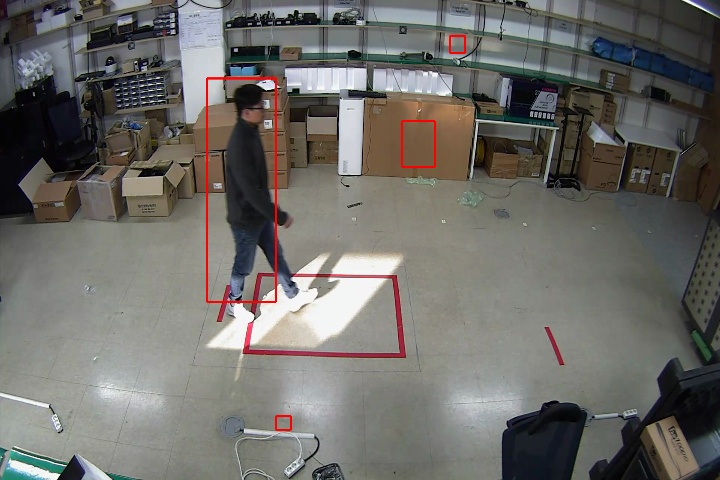
\includegraphics[width=0.25\linewidth]{Figures/1328_obj.jpg}
}\\
\subfloat[]
{
    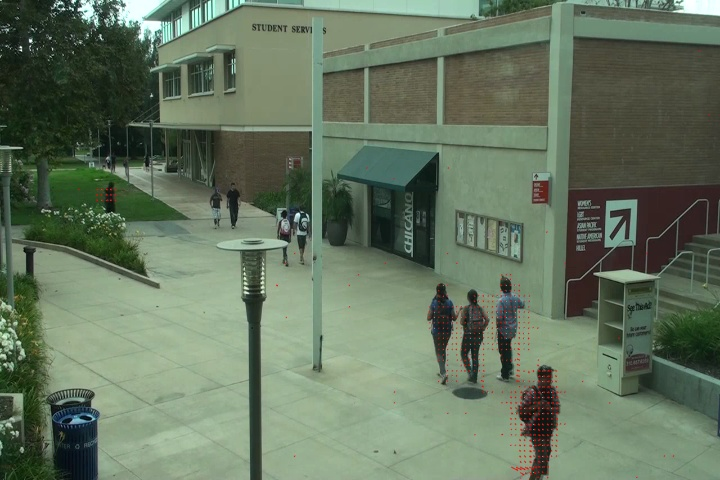
\includegraphics[width=0.25\linewidth]{Figures/38_mv.jpg}
}
\subfloat[]
{
    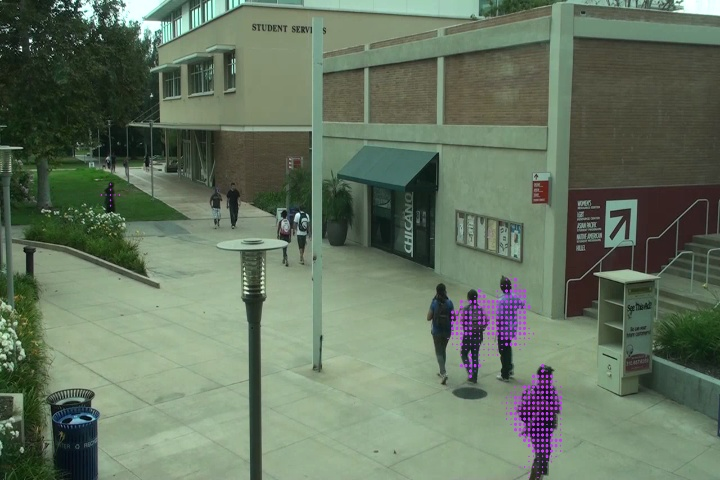
\includegraphics[width=0.25\linewidth]{Figures/38_occ.jpg}
}
\subfloat[]
{
    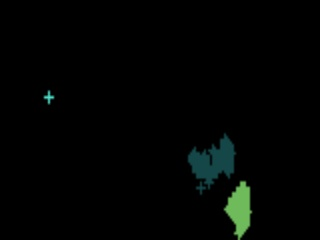
\includegraphics[scale=0.3]{Figures/38_res.jpg}
}
\subfloat[]
{
    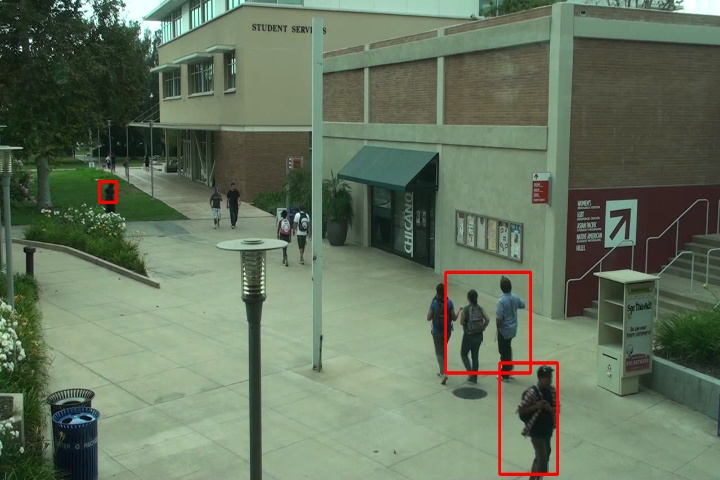
\includegraphics[width=0.25\linewidth]{Figures/38_obj.jpg}
}
\caption{Moving objects detection by the proposed method with two different video test sequences:(a,e) MV extraction; (b,f) Apply median filter; (c,g) Clustering MVs; (d,f) Blob detection.}
\label{fig:mvanalysis}
\end{figure*}
After clustering, the label list includes all candidate objects with various size, represented by different colors. Typically, the size of candidate object is followed by object size in the video frame. In small object dataset, objects are small when they have mean relative overlap (the overlap area between bounding box area and the image is) from 0.08\% to 0.58\%. Thus, we used a cluster threshold size to filter out the small clustered to the candidate lists as shown in Figure \ref{fig:filter}.\\
\begin{figure*}
\centering
 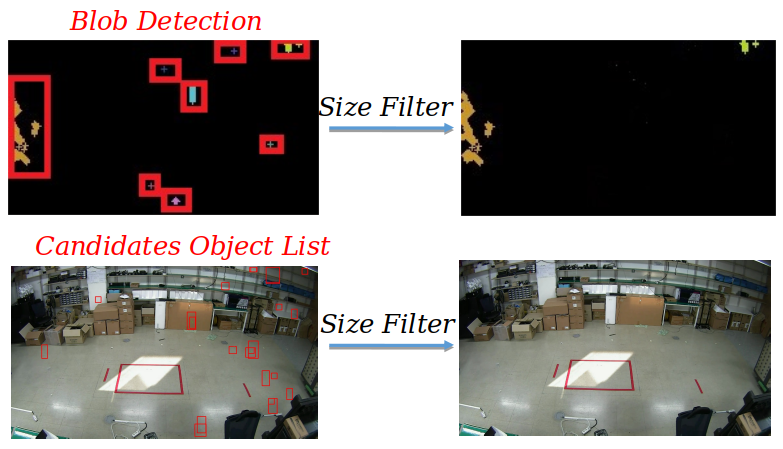
\includegraphics[width=1.0\linewidth]{Figures/filter.png}
 \caption{Motion size based Filtering}
 \label{fig:filter}
\end{figure*}
“After this process, the label list includes the moving objects and certain big MVs noises as shown in Figure \ref{fig:mvanalysis}(c,d). To eliminate these noises, we based the observation on the fact that noise motions because of lighting condition changes usually randomly occur without following a certain flow. Therefore, the tracking motion’s trajectories length is then used to classify the detected motion into the real motion or noise group. If the object tracking trajectory length is larger than a certain threshold, it indicates that the objects move as a flow and the time is sufficiently long to consider it as a real motion. Moreover, I-Frame does not apply motion estimation process, therefore, MV analysis process will be skipped for I-Frames. In order to overcome the discontinuously object detection process, the object tracking algotithm will also be applied to derive the moving object's bounding box in I-frame based on the last states in P-frames. Because the real object moves with a certain flow, the tracking
motion’s trajectories length is then used to classify the candidate
motions into the real motion or noise group, the IoU-based object tracking is applied to track motion because it is light-weight and widely tracking algorithm that calculates the overlap area between two bounding objects”(Nguyen Van Dien and Jaehyuk Choi, 2020, p.10). Note that this tracking was implemented and evaluated in some previous studies  \cite{sheu2019stam}, \cite{li2020hksiamfc}. 
\subsection{The low-complexity of overlapping based Moving Objects Tracking}
\label{subsec:1}
To apply the IoU-based object tracking, the detected clusters are normalized with a rectangle bounding box according to the cluster's size as shown in Figure \ref{fig:mvanalysis}(d,h). “The correlated regions are connected into blobs. Each blob is represented by its top-left and bottom-right corners, i.e.,  ($x_{1}, y_{1}, x_{2}, y_{2}$) may include one or many moving objects. Because the moving object's bounding box size and shape can be different comparatively frame by frame depending on motion vector intensity. Therefore, to track the moving object, the object matching algorithm which is based on the overlapped area calculation is applied. For example,  assuming that the existence of the real motion is continuous frame by frame. For each bounding box $B_{1}$ in the previous frame, we determine a bounding box $B_{2}$ at the current frame with the highest IoU score” (Nguyen Van Dien and Jaehyuk Choi, 2020, p.12). Note that IoU is attained by:\\
\begin{equation}
\label{eqn:2}
IoU(B_{1}\bigcap B_{2}) = \frac{\left \| B_{1}\bigcap B_{2} \right \|}{\left \| B_{1}\bigcup B_{2}  \right \|} =  \frac{\left \| B_{1}\bigcap B_{2} \right \|}{\left \| \left | B_{1} \right |  +  \left | B_{2} \right |  - B_{1}\bigcap B_{2} \right \|}
\end{equation} 
\begin{figure*}
\centering
 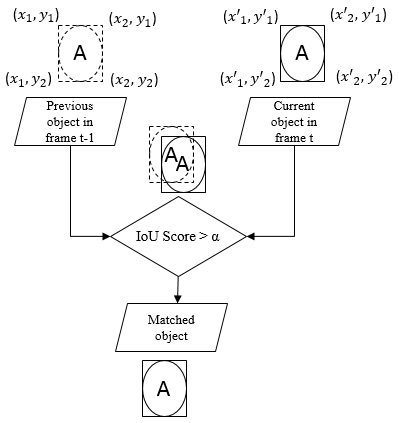
\includegraphics[width=0.4\linewidth]{Figures/iou.png}
 \caption{Object matching method}
 \label{fig:iou}
\end{figure*}
 As its definition in the Equation \ref{eqn:2}, “IoU is invariant to the scale, indicating that the similarity between two arbitrary shapes A and B is independent from the scale of their space. The IoU computation’s pseudo-code is given in Algorithm \ref{alg:iou_alg}. If two bounding boxes do not overlap, the IoU value will be 0 and if the IoU score is greater than a detection score threshold ($\alpha$), two bounding boxes are considered in same account (Figure \ref{fig:iou}). The detection score threshold is determined through experiments and depend on the object velocity as well as the distance between objects and camera. Therefore, the method is run with multiple times with different detection score thresholds to tune the best value for each application scenarios” (Nguyen Van Dien and Jaehyuk Choi, 2020, p.12). 
\begin{algorithm}
 \caption{ IoU calculation for two bounding boxes coordinates.}
 \label{alg:iou_alg}
\SetAlgoLined
\noindent\rule{16cm}{0.4pt}\\
\KwData{ Cordinates of the two bounding boxes.}
- First box: $A1(x_{1}, y_{1}), B1(x_{2}, y_{1}), C1(x_{2}, y_{2}), D1(x_{1}, y_{2})$\\
- Second box: $A2(x'_{1}, y'_{1}), B2(x'_{2}, y'_{1}), C2(x'_{2}, y'_{2}), D2(x'_{1}, y'_{2})$\\
  where $x_{1} \leq x_{2}, y_{2} \leq y_{1} and  x'_{1} \leq x'_{2}, y'_{2} \leq y'_{1}$.\\
\textbf{Calculation}: IoU value\\
- The area of first bounding box : $Area_{1} = (x_{2} - x_{1})\times (y_{1} - x_{2})$\\
- The area of second one : $Area_{2} = (x'_{2} - x'_{1})\times (y'_{1} - x'_{2})$\\
- The area of overlap: $Area_{overlap} = (max(x_{2},  x'_{2}) - min(x_{1},  x'_{1})) \times (max(y_{2},  y'_{2}) - min(y_{1},  y'_{1})) $\\
- $IoU value =\frac{Area_{overlap}}{Area_{1} +  Area_{2} - Area_{overlap}}$\\
\noindent\rule{16cm}{0.4pt}
\
\end{algorithm}
\section{ Performance Evaluated Model}
“Computing Resources of VA server is affected by many explicit factors. For example:  whether VA function is running, the complexity of VA function, video resolution, which kind of deep learning model used for VA function, how many cameras is serving. However, the primary factor and biggest effect is number of serving cameras and whether VA function is running. Because if  the VA server is in idle status, then other factors will be implicit. Let assume that we have a video test with N consecutive frames with K frames had the real motion (K<= N).  For each frame, VA server cost S and T unit  of average computing resource  for processing and skip frame case respectively.
For conventional method  of video analytics server, where T = S because all frames are processed , the computing resource average is:\\
\begin{equation}
\label{eqn:3}
Comp_{c}=S
\end{equation}
With our proposed method, the computing resource average during N frames  is calculated as the following equation:\\
\begin{equation}
\label{eqn:4}
Comp_{p}=\frac{(K*S+(N-K)*T)}{N}
\end{equation}
The performance ratio of two method is: \\
\begin{equation}
\label{eqn:5}
\frac{Comp_{p}}{Comp_{c}}=\frac{(K*S+(N-K)*T)}{N*S}=\frac{K}{N} + (1 - \frac{K}{N})*\frac{T}{S}
\end{equation}
if an object motion always appear in the video (K $\approx$ N), then: \\
\begin{equation}
\label{eqn:6}
 \frac{Comp_{p}}{Comp_{c}}\approx 1.
\end{equation}
In case of GPU consuming, when video analytic server skip a frame then T = 0 and:\\
\begin{equation}
\label{eqn:7}
\frac{Comp_{p}}{Comp_{c}} = \frac{K}{N}
\end{equation}
 If computing resource is CPU load and  network throughput ,  T is very small. Becuase T is used only for listening new connection, then: \\
\begin{equation}
\label{eqn:8}
 \frac{Comp_{p}}{Comp_{c}} \approx \frac{K}{N}
\end{equation}
”(Nguyen Van Dien and Jaehyuk Choi, 2020, p.12).
